\documentclass[11pt]{article}
\usepackage{graphicx}
\usepackage{amsmath,amssymb,amsthm}
\usepackage{epsfig}
\usepackage{cite}
\usepackage{subfigure}
\usepackage{graphics}
\usepackage{enumerate}
\usepackage{hyperref}
\usepackage{color}
\usepackage{multirow}
\usepackage{fancyhdr,textcase}
\usepackage{titlesec}
\usepackage{wrapfig}
\usepackage{lipsum} 
\usepackage[final]{pdfpages}
%\usepackage[a4paper, total={6.2in, 8.6in}]{geometry}
\allowdisplaybreaks
\usepackage{geometry}
 \geometry{
 a4paper,
 total={155mm,250mm},
 left=25mm,
right=25mm,
 top=20mm,
bottom=40mm,
 }
\setlength{\parindent}{0cm}
\allowdisplaybreaks
%\usepackage{scalerel}
\theoremstyle{plain}
\newtheorem{thm}{Theorem}[section]
\newtheorem{lemm}[thm]{Lemma}
\theoremstyle{definition}
\newtheorem{exm}[thm]{Example}
\newtheorem{defi}[thm]{Definition}
\newtheorem{cor}[thm]{Corollary}
\newtheorem{claim}[thm]{Claim}
\newtheorem{rmk}[thm]{Remark}
\newtheorem{prop}{Proposition}
\newtheorem{prob}{Problem}
\newcommand{\defeq}{\stackrel{\text{def}}{=}}
\newtheorem{conj}[thm]{Conjecture}
\newcommand{\norm}[1]{\left\lVert#1\right\rVert}
\newcommand\T{\rule{0pt}{3ex}}
\newcommand\B{\rule[-3ex]{0pt}{0pt}}
\titleformat{\paragraph}{\normalfont\normalsize\bfseries}{\theparagraph}{1em}{}
\titlespacing*{\paragraph}{0pt}{3.25ex plus 1ex minus .2ex}{1.5ex plus .2ex}

\setcounter{secnumdepth}{4}
\setcounter{tocdepth}{4}

%\newcommand\reallywidehat[1]{%
\DeclareMathOperator{\re}{Re} \DeclareMathOperator{\im}{Im}
\DeclareMathSymbol{\C}{\mathalpha}{AMSb}{"43}
\DeclareMathOperator{\supp}{supp}
%\newcommand{\supp}{supp}

\author{Valmir Bucaj, PhD}
\date{}
\pagestyle{fancy}
\markright{MA477 -- Intro to ML\\ AY20-2 USMA, West Point}

%\markleft(Cadet}
%\setlength\parindent{0pt}
\usepackage{mathtools}
\DeclarePairedDelimiter\ceil{\lceil}{\rceil}
\DeclarePairedDelimiter\floor{\lfloor}{\rfloor}
\begin{document}

\title{\begin{figure}[h!]

\includegraphics[width=30mm]{logo.png}
\end{figure}\vspace{-1cm}\textsc{MA477\\ Theory and Applications of Data Science \\ -- Course Outline}}

\maketitle

\tableofcontents
\thispagestyle{fancy}

\newpage

\begin{figure}[h!]

\includegraphics[width=30mm]{logo.png}
\end{figure}
\begin{center}
\vspace{-3cm}
DEPARTMENT OF THE ARMY\\
{\bf UNITED STATES MILITARY ACADEMY}\\
West Point, New York 10996
\end{center}
\vspace{.5cm}
{\bf \tiny{REPLY TO \\ ATTENTION OF}}
\vskip 12pt
MADN-MATH	
\vspace{.2cm}


\section{Instructional Memorandum $\#$ 477-20-02}

\begin{center} \textsc{MA477 -- Theory and Applications of Data Science} \end{center}

\subsection{Purpose}

This memorandum specifies materials, describes the goals and objectives, and announces policy and procedures for MA477 during AY 20-02.

\subsection{Instructor Info}

Instructor: Dr. Valmir Bucaj\\
Office Nr.: TH224\\
Ext: 7460\\
Email: valmir.bucaj$@$westpoint.edu

\subsection{Course Website}

All of the materials for this course will be published and made available in our course website, which may be found in the link below:
\vskip 12pt

\href{https://vbucaj.github.io/MA477-course/}{Course Website URL}


\subsection{Textbooks and Supporting Materials}

For this course you are required to have the following two textbooks:

\begin{enumerate}[(1)]
\item Machine Learning: An Applied Mathematics Introduction by Paul Wilmott
\item An Introduction to Statistical Learning by G. James, D. Witten et.al.
\end{enumerate}

While you are welcomed to purchase both books, the second one may be downloaded for free from the author's webpage by  \href{http://faculty.marshall.usc.edu/gareth-james/ISL/}{Clicking Here!}.
\vskip 12pt

{\bf Extra Resources}

You are also strongly encouraged to create an account with Data Camp and use it as a supporting resource. To open an account follow the link \href{https://www.datacamp.com/}{DataCamp}. In addition to posting the notes on our course website, I will also post all of the JupyterNotebooks on my GitHub page, which you may find  \href{https://github.com/vbucaj/lecture-notes}{HERE!}.


\subsection{Technology Requirements}

For the entirety of this course we will exclusively be using Python as our programming language. 

\vskip 8pt

While you are welcome to use a desktop Python IDE, you are strongly encouraged to use JupyterNotebooks, as this is what we will almost exclusively use throughout the course. You are strongly suggested to download Anaconda. 

\vskip 8pt

Anaconda is a free Python distribution which contains over 1500 open source packages, as well as Python itself, for performing scientific computation. In this case we will use this distribution, its packages, the Spyder IDE, and Jupyter Notebooks (all of this is included in this one download / install). 

\vskip 8pt

To install Anaconda follow the steps below:

\begin{enumerate}[(1)]
\item \href{https://www.anaconda.com/distribution/}{Click on the Anaconda website!}
\item Download the file that has Python $3$.xx
\item In the Programs Folder or Start-up Menue find Anaconda 3 folder
\item Click on Anaconda Navigator
\item Locate JupyterNotebook and click Launch
\end{enumerate}

You are also required to open a GitHub account. To do so \href{https://github.com/}{Click Here!}

\subsection{Course Goals}

The purpose of this course is to build a solid foundation in the theoretical and applied aspects of Machine Learning as well as an appreciation for its vast applications in a variety of fields across many domains. It will introduce a variety of supervised and unsupervised machine learning techniques with applications in Python.

\subsection{Course Evaluation Plan}

Final course grades will follow department standing guidelines. Cadets can view their performance on all graded events in CIS. 
\vskip 8pt
The weight of each graded portion will roughly be as follows:


\begin{table}[!h]
\begin{center}
\scalebox{1.2}{
\begin{tabular}{|c|c|c|c|}
\hline
{\bf Event}& {\bf Count } &{\bf Points }& {\bf Weight (\%) }\\
\hline
Exercises &3-5&150&15\\
\hline
Quizzes &3-5&200&20\\
\hline
Mini-Projects &5-7&400&40\\
\hline
TEE &1&250&25\\
\hline
\multicolumn{2}{|c|}{\bf Total}&1000&100\\
\hline

\end{tabular}}
\end{center}
\end{table}

\subsubsection{Exercises}

After completing most sections from the module {\bf Python for Data Analysis and Visualization}, you will be assigned a short set of {\bf JupyterNotebook} Exercisses. The purpose of these exercises will be to reinforce the concepts taught in class as well as give students an opportunity to go beyond what was taught in class. 

\subsubsection{Quizzes}

These will be $15-20$ minute in-class concept quizzes. They will exclusively focus on theoretical concepts covered up to that point, and as such technology will not be permitted. The rough idea is for the first quiz to be administered after the section on {\bf Regression Models}, the second after the section on {\bf Classification Models}, the third after the chapter on {\bf Unsupervised Learning Methods}, the fourth after {\bf Neural Networks} and possibly a fifth somewhere in the mix as we see fit. 

\subsubsection{Mini-Projects}

These will be individual mini JupyterNotebook Projects, and they will be assigned after most, if not each, of the Machine Learning Methods covered in class. For example, there will be a mini-project about the Python for Data Analysis and Visualization module, another one about the K-NN Regressor, and another about Linear Regression, and so on. 

\vskip 8pt

The purpose of these mini-projects is to provide students wit an opportunity to:

\begin{itemize}
\item Utilize the knowledge acquired in class up to that point
\item  Independently investigate a problem
\item Reinforce the concepts already learned
\item Be creative and show originality in thought and in implementing various ML tools.
\end{itemize}

I strongly believe that constructive competition drives progress, so in line with this mantra, the mini-projects will be of a competitive nature, as well, where your individual ranking in the competition will determine your score on the project! More specific details will be issued with each project! 

\subsubsection{TEE}

The TEE for this course will consist of two parts:
\begin{enumerate}[1)]
\item An oral presentation
\item A questions and answers session
\end{enumerate}

At least one week before the end of the semester you will be assigned a project with specific guidelines which will consist of your TEE for the course. On the day of the TEE  you will each give a 10-15 minute presentation which will be followed up by a 10-15 minute QA session. 

\subsection{Professional Development}

To help you achieve the student growth goals stated above, we have the following expectations for your efforts.  

\begin{enumerate}[a.]
\item {\bf Data Science is not a Spectator Sport.} To be successful in Data Science, we have to do the work. Often, we fall into the trap of seeing a professor or peer do a problem and think “Oh, that’s how you do it” and we move on. That approach will not be good enough in this course. We will not grade you on your ability to recognize the right answer, rather on your ability to produce it. To summarize a key point from Malcolm Glidewell’s book, Outliers, it takes many repetitions to get good at something. Do the reps. There’s simply no substitute.

\item {\bf Be Prepared.} Cadets have full days. Spending time with the material before class will enable your days to be more efficient and more productive. Some material in MA477 is material you may have seen in other courses. Some is relatively straight forward. Other material is challenging. With your prior preparation, your professors can provide light(er) treatment on the material you’ve seen before and/or is easily attainable and heavily weight class time toward the more challenging concepts. We can help you get more reps on the hard material, enabling your excellence now and in the future.

\item {\bf Build a Team.} Ray Kroc, the founder and first CEO of McDonald’s said “All of us is better than any of us.” West Point and the Army are team activities. Build your Data Science team and use it to maximize your success. Study together, do exercises together, and brief each other. Seek additional resources when needed, including additional instruction (AI) from your professor. The primary purpose of AI is to address specific questions that you may have; it is not a lesson reteach.

\item {\bf Show Your Pride.} Understand what the expectations are for each task you are given and meet those expectations to the best of your ability. Do your best work. Do it neatly. 

\item {\bf Be on Time.}  When you are given a deadline, meet it.
\end{enumerate}


\subsection{Classroom Rules}

All cadets are expected to maintain proper military bearing and appearance during instruction in accordance with appropriate regulations.

\begin{enumerate}[a.]
\item Respect others’ rights in the classroom. No profanity, unprofessional jokes, or unprofessional computer items (audio or visual). If what you are doing is distracting anyone else in the class, what you are doing is wrong.
\item Store backpacks in the hallway.
\end{enumerate}

\subsection{Scholarship}

This course is designed to build upon your previous instruction in mathematics and statistics as well as to explore new concepts.  It is therefore appropriate (and you are encouraged) to consult sources of information beyond the course text.  In doing so, keep in mind the standards of scholarly work.  Documentation of your effort should follow the guidance contained in Documentation of Written Work, published by the Dean’s Office, June 2015.  If you are not sure about how or when to document a source, discuss the matter with your instructor prior to submitting your work.

\subsection{Your Learning.}

Finally, this is your education. You must take responsibility for your own learning and participate as an active learner.  Your professor is here as a resource to help guide you through the educational experience this course offers, but he is only one resource.  There are many others.  The quantitative reasoning and problem solving skills that you continue to develop in this course will serve you in the future regardless of your major as a Cadet or your branch as an officer.  Use this opportunity to develop confidence, competence, and good habits of mind.  These are the ends which we will use mathematics and machine learning as a means to reach.

\subsection{Chain of Command}

The Department of Mathematical Sciences has an open door policy. Your initial attempt to address problems or concerns should go through the chain of command. However, if you are uncomfortable addressing an issue with your instructor, please approach any individual in the chain. If you have any concerns related to respect in the classroom, unprofessional behavior, or sexual assault or harassment, please feel free to contact the Department Head directly. Below is the chain of command for MA477:

\begin{enumerate}[a.]
\item {\bf Your Instructor:} Dr. Valmir Bucaj
\item {\bf Elective Mathematics Program Director:} COL Watts, TH239A, (845) 938-2276
\item {\bf Head of the Department:} COL Tina Hartley, TH 238, (845) 938-5285
\end{enumerate}
\newpage
\subsection{Course Calendar}

\begin{figure}
 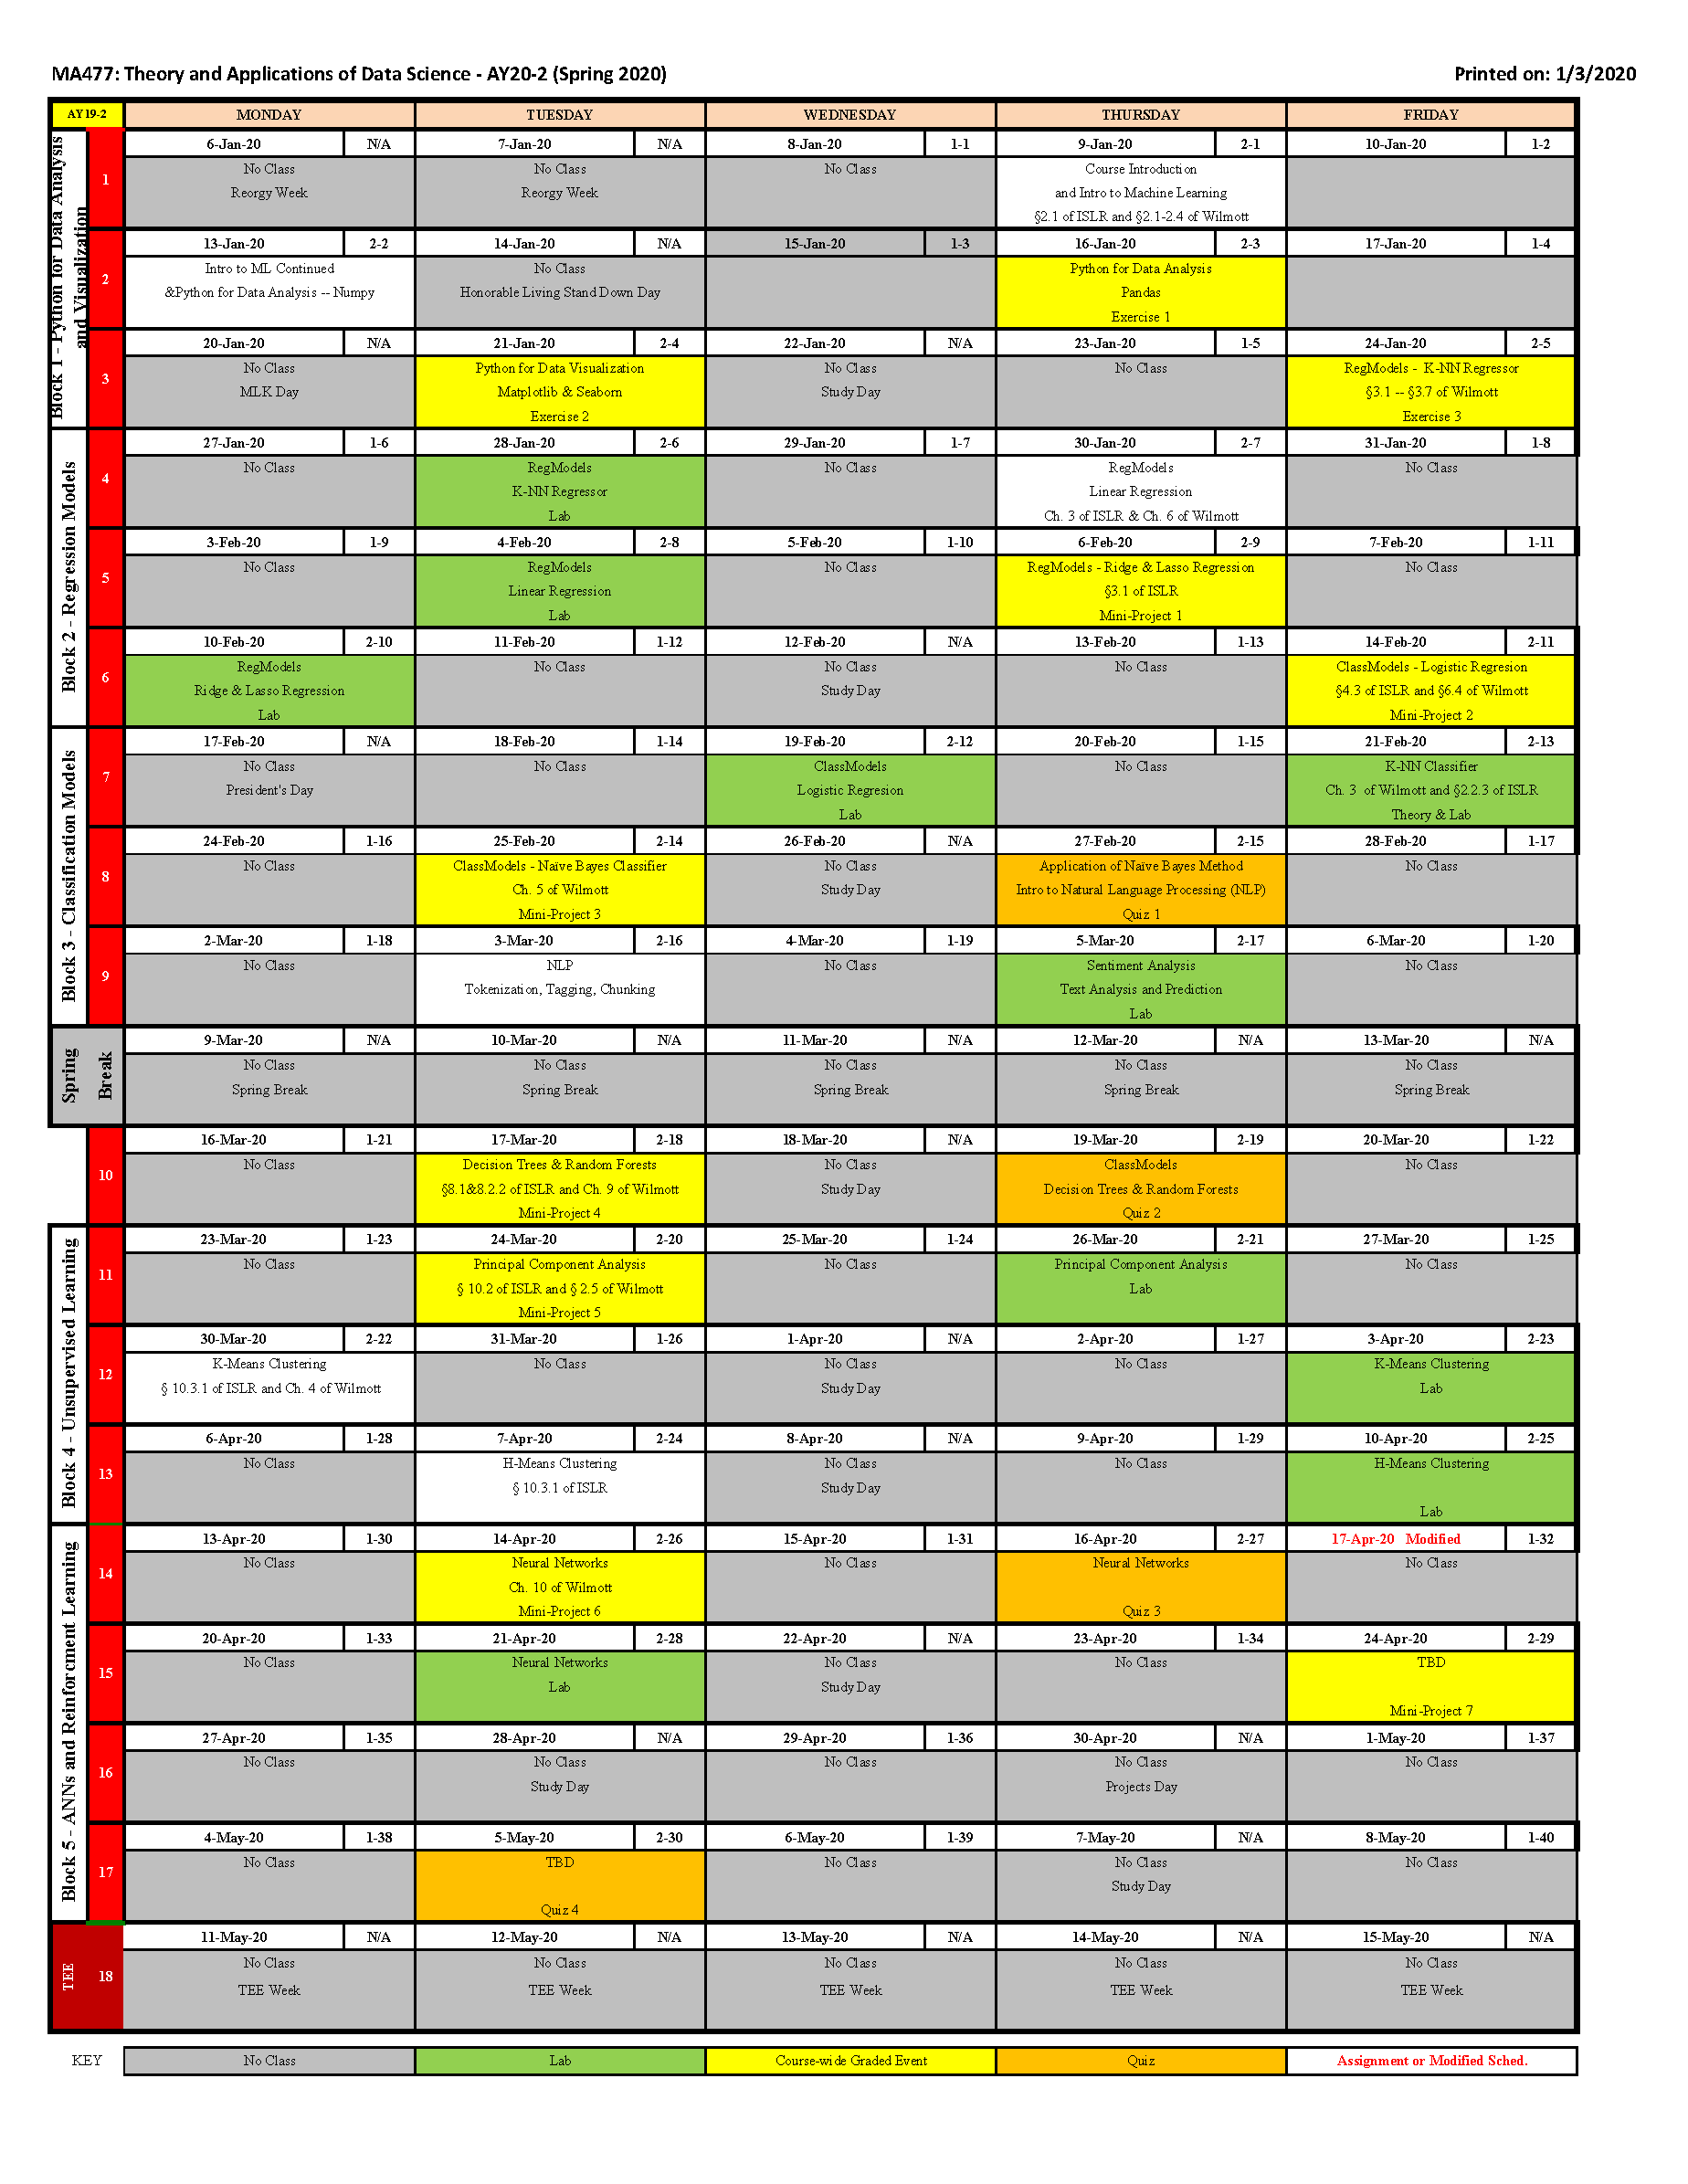
\includepdf[pages=-, width=1.15\textwidth]{Calendar}
\end{figure}

\newpage
\section{Intro to Machine Learning -- A Brief Overview}

\subsection{What is ML?}

Suggested Reading:
\begin{itemize}
\item Section 2.1 of \cite{ISLR} 
\item Chapter 1 and Sections 2.1 -- 2.4 of \cite{wilmott}.
\end{itemize}

\subsubsection{Estimating the relationship between {\it predictor} and {\it response}}

\subsubsection{Prediction Accuracy vs. Model Interpretability}

\subsubsection{Supervised vs. Unsupervised Learning}

\subsubsection{Regression vs. Classification Models}

\subsection{Assessing Model Accuracy}

Suggested Reading:

\begin{itemize}
\item Sections 2.7 and 2.11 of \cite{wilmott}
\item Sections 2.2.1 and 2.2.2 of \cite{ISLR}
\end{itemize}

\begin{enumerate}[(a)]
\item Classification Setting
\begin{itemize}
\item Confusion Matrix and ROC Curve
\item Cross-Validation
\end{itemize}

\item Regression Setting
\begin{itemize}
\item Mean Squared Error
\end{itemize}
\end{enumerate}

\subsection{Bias - Variance Trade-Off}

\newpage
\section{Python for Data Analysis and Visualization}

In this chapter we will talk



\subsection{Numpy}
\subsubsection{Numpy Arrays and Indexing}

\subsubsection{Numpy Operations}

\vspace{1cm}

\subsection{Pandas}

\subsubsection{Series}

\subsubsection{Data Frames}

\subsubsection{Missing Data, Groupby, and Basic Operations}

\subsubsection{Merging, Joining, and Concatenating}

\subsubsection{Reading and Writing Data}

\vspace{1cm}

\subsection{Matplotlib}

\subsubsection{Basic Plotting Methods}

\subsubsection{Object Oriented Plotting Methods}

\vspace{1cm}

\subsection{Seaborn}

\subsubsection{Distribution and Categorical Plots}

\subsubsection{Matrix Plots}

\newpage 

\section{Supervised Learning Methods}

\subsection{Regression Models}

\subsubsection{K-Nearest Neighbors Regressor}

Suggested reading:

\begin{itemize}
\item Chapter 3 of \cite{wilmott}
\end{itemize}

\subsubsection{Linear Regression -- Least Squares}

Suggested Reading:

\begin{itemize}
\item Chapter 3 of \cite{ISLR}
\item Sections 6.1--6.3 of \cite{wilmott}
\end{itemize}

\subsubsection{Ridge and Lasso Regression}

Suggested Reading:

\begin{itemize}
\item Section 6.3 of \cite{ISLR}
\end{itemize}


\subsubsection{(Optional) Random Forest Regressor}


\vspace{1cm}
\subsection{Classifications Models}

Suggested Reading:

\begin{itemize}
\item Sections 4.1 and 4.2 of \cite{ISLR}
\end{itemize}

\subsubsection{Logistic Regression}

Suggested Reading:

\begin{itemize}
\item Section 4.3 of \cite{ISLR}
\item Sections 6.4 and 6.5 of \cite{wilmott}
\end{itemize}

\subsubsection{K-Nearest Neighbors Classifier}

Suggested reading:

\begin{itemize}
\item Chapter 3 of \cite{wilmott}
\item Section 2.2.3 of \cite{ISLR}
\end{itemize}


\subsubsection{Naive Bayes Classifier}

Suggested Reading:

\begin{itemize}
\item Chapter 5 of \cite{wilmott}
\end{itemize}

\subsubsection{Natural Language Processing (NLP)}

\begin{enumerate}[I.]
\item Overview  of the Natural Language Tool Kit (NLTK)
\begin{itemize}
\item Counting Text
\item Frequency Distribution
\item Bigrams
\end{itemize}
\item Overview of Regular Expressions (RegExp)
\item Tokenization
\item Tagging
\item Chunking

\end{enumerate}




\subsubsection{Decision Trees and Random Forests}

Suggested Reading:

\begin{itemize}
\item Sections 8.1 and 8.2.2 of \cite{ISLR}
\item Chapter 9 of \cite{wilmott}
\end{itemize}

\subsubsection{(Optional) Support Vector Machine Classifier (SVC)}


\newpage

\section{Unsupervised Learning Methods}

Suggested Reading:

\begin{itemize}
\item Section 10.1 of \cite{ISLR}
\end{itemize}

\subsubsection{Principal Component Analysis}

Suggested Reading:
\begin{itemize}
\item Section 10.2 of \cite{ISLR}
\item Section 2.5 of \cite{wilmott}
\end{itemize}

\subsubsection{K Means Clustering}

Suggested Reading:

\begin{itemize}
\item Section 10.3.1 of \cite{ISLR}
\item Chapter 4 of \cite{wilmott}
\end{itemize}

\subsubsection{H-Means Clustering}

Suggested Reading:
\begin{itemize}
\item Section 10.3.2 of \cite{ISLR}
\end{itemize}


\subsubsection{(Optional) T-distributed Stochastic Neighbor Embedding (t-SNE)}


\newpage
\section{Neural Networks}

Suggested Reading:
\begin{itemize}
\item Chapter 10 of \cite{wilmott}
\end{itemize}

\newpage


\section{Reinforcement Learning}
Suggested Reading:
\begin{itemize}
\item Sections 11.1 -- 11.17 of \cite{wilmott}
\end{itemize}

\newpage
\section{(Optional) Recommender Systems}



\newpage

\begin{thebibliography}{9}
%\bibliographystyle{plain}

\bibitem{ISLR}

G. James, D. Witten, T. Hastie, R. Tibshirani {\it An Introduction to Statistical Learning} Springer, 2014.

\bibitem{wilmott}

P. Wilmott. {\it Machine Learning: An Applied Mathematics Introduction}. Panda Ohana Publishing. 2019.



\end{thebibliography}


\end{document}